\chapter{Related Work}

\section{Pose Estimation}
first: single images only, no video
\subsection{Pictoral Structure Framework}
%TODO: Write a little bit about original paper
structure defined by parts (limbs) connected together. connections using "springs". deformable structure.
Minimize energy function. See \cite{zhu_articulated_2016}

% ------ GENERAL OBJECT RECOGNITION FRAMEWORK ----------
%TODO: simplified version of statistical model
%   TODO: not specifically pose but general object recognition
Taking the energy minimization problem presented in \cite{fischler_representation_1973}, the authors transform it into a statistical framework.
One advantage is that the parameters can then be estimated utilizing training examples, similar to the principles of learning presented in \ref{sec:neural_networks}.
Also, it is trivial to get multiple solutions to the minimization problem by sampling the posterior distribution as opposed to a single solution with the energy minimization approach.

The authors model the problem as follows.
Let $p(L \mid I, \theta)$ be the desired posterior distribution, where $L$ is the set of object configurations (like object positions, rotations etc.), $\theta$ is a set of model parameters and $I$ is the image.
When applying Bayes' formula, one can express the posterior as 

\begin{equation}
    p(L \mid I, \theta) \propto p(I \mid L, \theta) p(L \mid \theta)
\end{equation}

The likelihood $p(I \mid L, \theta)$ is approximated as $\prod_{i=1}^n p(I \mid l_i, \theta_i)$.
This approximation, however, is bad if recognized parts overlap, which is often the case when detecting human limbs.
The authors tackle this problem by sampling multiple times from the posterior and evaluating them using a separate measurement.

To approximate the prior distribution $p(L \mid \theta)$ the authors utilize the joint distribution of a tree structured Markov random field.
The vertices are modeled by $l_i$ and the edges show connections between the different parts. 
They set the denominator to $1$ because they argue that it can be constant if only relative position between parts is of importance.

\begin{equation}
    \begin{split}
        p(L \mid \theta) 
        &\propto \frac{\prod_{(i,j) \in E} p(l_i, l_j \mid \theta)}{\prod_{i \in V} p(l_i \mid \theta)^{\text{deg} ~ v_i -1}} \\
        &\propto \prod_{(i, j) \in E} p(l_i, l_j \mid \theta)
    \end{split}
\end{equation}

%TODO: exlain why equivalent to minimizing energy function

After presenting the statistical framework for general object recognition tasks, the authors explain their approach to pose estimation using this framework.
First, they specify that the input image needs to be a binary image where the person is separated from the background.
Then, the objective is to maximize the number of foreground pixels covered by the detected limbs in their calculated configuration.
A visualization of this process can be seen in \fref{fig:felzenszwalb-overview}.

\begin{figure}[htb!]
    \centering
    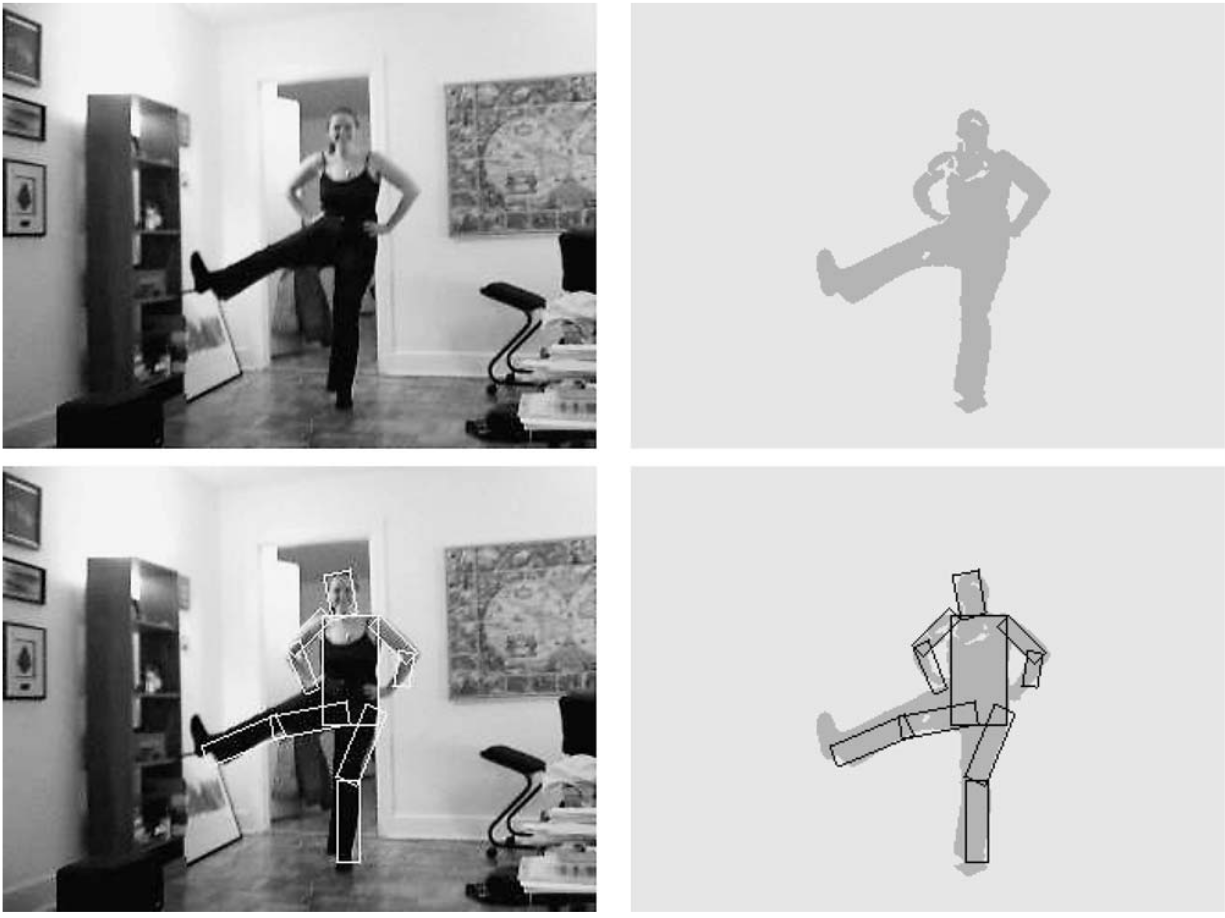
\includegraphics[width=0.8\textwidth]{felzenszwalb-overview.png}
    \caption{Overview of pose matching algorithm. \textbf{Upper left}: Original image. \textbf{Upper right}: binary image where foreground pixels (containing the human figure) are separated from the background. \textbf{Lower right}: One result from matching the limb rectangles to maximize the amount of foreground pixels covered. \textbf{Lower left}: Final result with estimated pose layered on top of original image. Image taken from \cite{felzenszwalb_pictorial_2005}}
    \label{fig:felzenszwalb-overview}
\end{figure}

The authors model the human pose as a collection of $10$ different parts. 
Two parts per arm and leg as well as one torso and one head part \fref{fig:felzenszwalb-overview}.
Each limb configuration $l_i = (x_i, y_i, s_i , \varphi_i)$ contains the $x$ and $y$ coordinate of the center of the rectangle.
In addition, $s_i \in [0,1]$ defines the length of the rectangle and $\varphi_i$ its rotation.
The width is fixed.

To model $p(I \mid l_i, \theta_i)$ they use the following formula which utilizes $\theta_i = (q_1, q_2)$.
$q_1$ is the probability of pixel inside $l_i$ being a foreground pixel whereas $q_2$ is the probability of pixels closely around $l_i$ being foreground pixels.
The area around $l_1$ is referred to as $area_2$ whereas the area of $l_i$ is referred to as $area_1$.
$count_i$ referres to the number of foreground pixels in $area_i$ and $t$ is the total number of pixels in the image.

\begin{equation}
    \begin{split}
        p(I \mid l_i, (q_1, q_2)) = &q_1^{count_1} * (1 - q_1)^{(area_1 - count_1)} \\ 
        &* q_2^{count_2} * (1 - q_2)^{(area_2 - count_2)} \\ 
        &* 0.5^{(t - area_1 - area_2)}
    \end{split}
\end{equation}

Also, they smooth the distribution to prevent peaks by using the principle of annealing with a constant factor $T$.
This is important because a distribution with strong peaks is more likely to return similar results when sampling.
As discussed earlier, this sampling is needed because of the approximation the authors used and its problem with overlapping limbs.  A distribution with too strong peaks would not allow for sufficiently different pose samples.

$\theta_i$ is then estimated using mean values from annotated training data points while $T$ is set to $10$.

\begin{equation}
    p(I \mid l_i, \theta_i) \propto p(I \mid l_i, \theta_i)^{\frac{1}{T}}
\end{equation}

\begin{figure}[htb!]
    \centering
    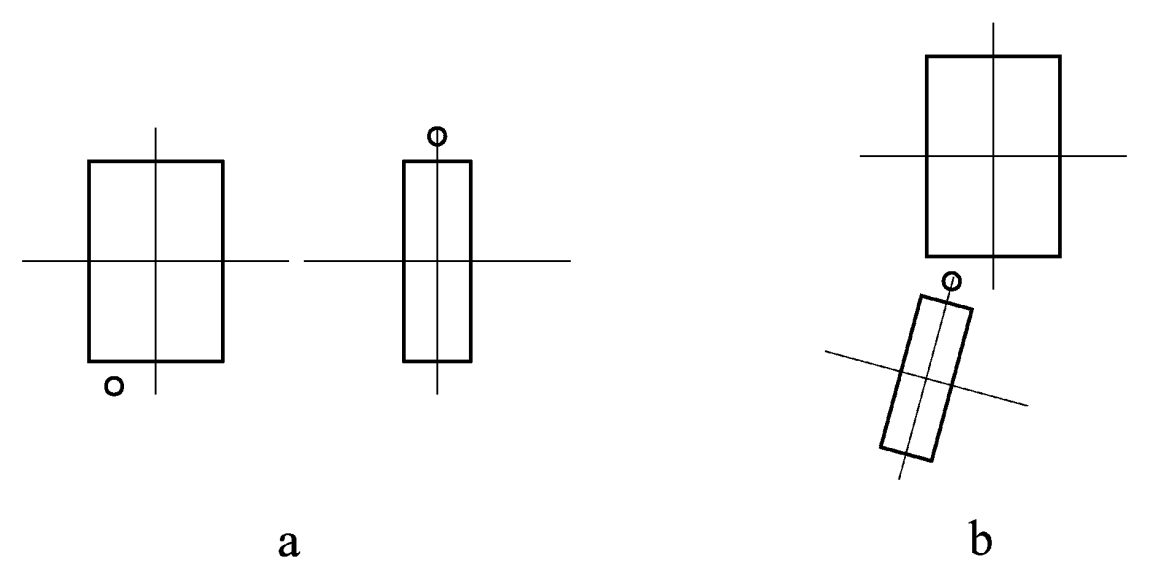
\includegraphics[width=0.8\textwidth]{limb-connection.png}
    \caption{Visualization of connecting limbs. \textbf{a}: Two limbs in their own coordinate system. The circle indicate connection joints. \textbf{b}: Possible, anatomically plausible connection. Image taken from \cite{felzenszwalb_pictorial_2005}}
    \label{fig:limb-connection}
\end{figure}

For the prior, consider the visualization in \fref{fig:limb-connection}.
Given the local center points $(x_i, y_i)$ for each limb $l_i$, the authors calculate $(\hat{x}_i, \hat{y}_i)$ using free parameters $(x_{ij}, y_{ij})$ like this:

\begin{equation}
    \begin{bmatrix}
        \hat{x}_i \\ 
        \hat{y}_i
    \end{bmatrix}
    =
    \begin{bmatrix}
        x_i \\ 
        y_i
    \end{bmatrix}
    + s_i R_{\varphi_i}
    \begin{bmatrix}
        x_{ij} \\ 
        y_{ij}
    \end{bmatrix}    
\end{equation}

$R_{\varphi_i}$ is a matrix which rotates around the origin for $\varphi_i$ radiants.
This projection then gets used in the prior distribution formula:

\begin{equation}
    \begin{split}
        p(l_i, l_j \mid \theta) 
        &= p(l_i, l_j \mid c_{ij}) \\
        &= N((\hat{x}_i - \hat{x}_j), 0, \sigma_x^2) \\
        &* N((\hat{y}_i - \hat{y}_j), 0, \sigma_y^2) \\
        &* N((s_i - s_j), 0, \sigma_s^2) \\
        &* M((\varphi_i - \varphi_j), \varphi_{ij}, k)
    \end{split}    
\end{equation}

Except for the last part of the equation, all distributions are Gaussian with a mean of $0$.
The last distribution is a von Mises distribution, given by

\begin{equation}
    M(\theta, \mu, k) \propto \exp (k \cdot \cos (\theta - \mu))
\end{equation}

Using this distribution, the difference between the two angles is measured with regards to the optimal orientation $\varphi_{ij}$.
A von Mises distribution can be thought of as a normal distribution around a circle, which is why the authors use it for periodic input like gradients.
The parameter $k$ determines how strong the peak at $\varphi_{ij}$ should be or, in other words, how constrained the joints should be. 

The prior parameters $c_{ij}$ are thus given by $c_{ij} = (x_{ij}, x_{ji}, y_{ij}, y_{ji}, \sigma_x, \sigma_y, \sigma_s, \varphi_{ij}, k)$ and are estimated using maximum likelihood estimation.

% ----- Short evaluation
The authors merely provide example images instead of a quantitative analysis.
This is most likely because of the lack of benchmark data sets at the time of writing their thesis.
They labeled $10$ images by hand and used these to estimate the parameters.
Then, for each of their unlabeld test images, they sampled $200$ poses and calculated the Chamfer distance, which measures the binary correlation.
The best pose with regards to the Chamfer distance is then returned.
Some example images can be seen in \fref{fig:pictoral-examples}

\begin{figure}[htb!]
    \centering
    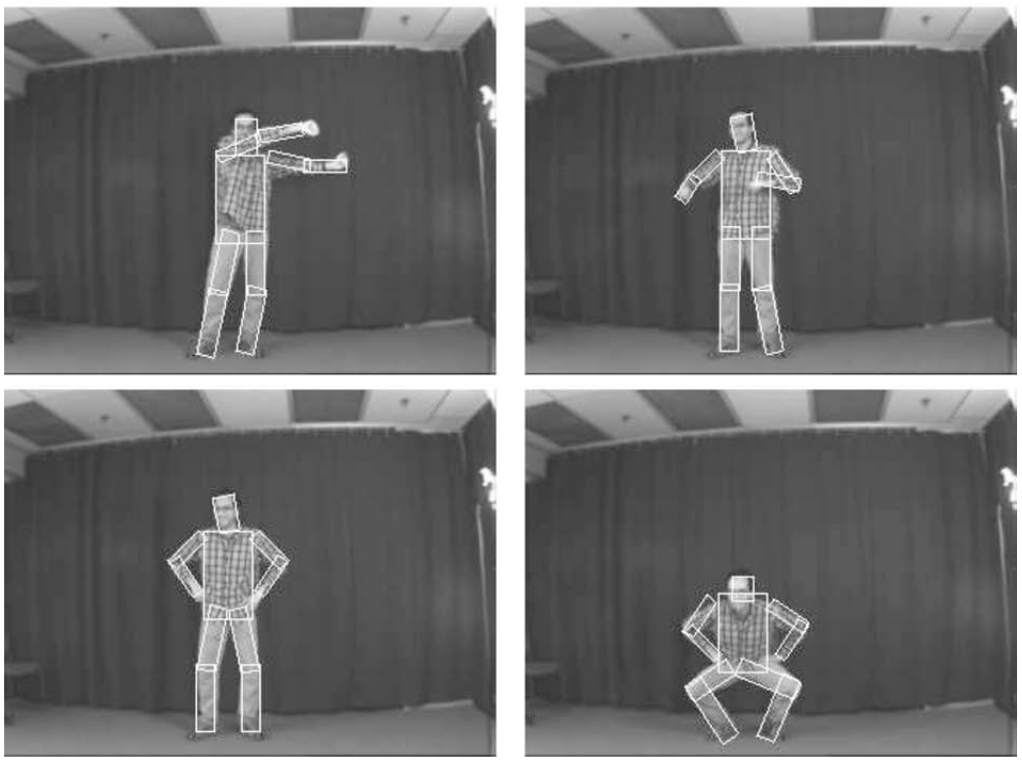
\includegraphics[width=0.8\textwidth]{pictoral-examples.png}
    \caption{Example of poses estimated by the statistical framework. Image taken from \cite{felzenszwalb_pictorial_2005}.}
    \label{fig:pictoral-examples}
\end{figure}

\begin{itemize}
    \item Pictoral Structures for Object Recognition \cite{felzenszwalb_pictorial_2005}
    \item Articulated pose estimation with flexible mixture-of-parts \cite{yang_articulated_2011}
    \item An approach to pose-based action recognition \cite{wang_approach_2013}
\end{itemize}

\subsection{Deep Learning Methods}
\begin{itemize}
    \item DeepPose \cite{toshev_deeppose:_2014}
    \item Stacked Hourglass \cite{newell_stacked_2016}
    \item Convolutional Pose Machine \cite{wei_convolutional_2016}
    \item Thin-Slicing Network \cite{song_thin-slicing_2017}
\end{itemize}

\section{Video-based Human Action Recognition}
\subsection{Shallow Methods}
\begin{itemize}
    \item Learning Realisitic Human Actions from Movies \cite{laptev_learning_2008}
\end{itemize}

\subsection{Deep Methods}
\begin{itemize}
    \item MiCT \cite{zhou_mict:_2018}
\end{itemize}